% Global South AI Safety Hackathon 2026 — Official submission template (LaTeX)
% Compile: pdflatex report.tex  (from this directory)
\documentclass[10pt]{article}

\usepackage[utf8]{inputenc}
\usepackage[T1]{fontenc}
\usepackage[english]{babel}
\usepackage{mathptmx}
\usepackage[letterpaper,margin=1in]{geometry}
\usepackage{graphicx}
\usepackage{booktabs}
\usepackage{array}
\usepackage{tabularx}
\usepackage{enumitem}
\usepackage[hidelinks]{hyperref}

\newcolumntype{L}[1]{>{\raggedright\arraybackslash}p{#1}}
\setlength{\parskip}{0.35em}
\setlength{\parindent}{0pt}
\setlength{\emergencystretch}{2em}

% ---------------------------------------------------------------------
\begin{document}

% --- Title block (matches Word template) ---
\begin{center}
{\Large\bfseries HAZE: Adversarial Multi-Agent Scrutiny for\\
Vulnerability Detection\par}
\vspace{0.8em}
\begin{tabular}{@{}c@{}}
Samuel Blanco \\
AI Safety México \\[0.4em]
Samuel Díaz \\
AI Safety México \\[0.4em]
Axel Morales \\
AI Safety México \\[0.4em]
Alex Novelo \\
AI Safety México \\
\end{tabular}

\vspace{0.6em}
{\small With Apart Research}

\vspace{0.4em}
{\small
\textbf{Region:} Latin America (AISMX --- México)\\
\textbf{Track:} AI Security\\
\textbf{Sub-track:} Pipeline security (API, cloud)\\
\textbf{Secondary track:} Responsible AI\\
\textbf{Secondary sub-track:} Hallucination mitigation \& behavioral audit
}
\end{center}

\vspace{0.3em}
\noindent\rule{\textwidth}{0.4pt}
\vspace{0.3em}

% --- Abstract ---
\noindent{\bfseries Abstract}\par
\vspace{0.2em}
Single-agent LLM auditors treat every prompt as a hunt for a flaw---and often
\textbf{manufacture findings} to satisfy it (Perez et al., 2022). We built
\textbf{HAZE} (*Hallucination-Aware Zero-sum Examination*), a red-teaming protocol
where four LLM roles debate under AI Safety via Debate (Irving et al., 2018):
prosecution and defense cross-examine over a code artifact; an \textbf{isolated
judge} rules only on what survived refutation. \textit{Core claim:} single-agent
auditors ask ``is there a bug?''; HAZE asks ``did this accusation survive
refutation?'' We evaluate on 10 CVEs $\times$ \{vulnerable, patched\} = 20
artifacts (3 repeats, majority verdict, Wilson 95\% CIs, McNemar test).
\textbf{Primary result (Phase~1, \texttt{VULNERABLE}/\texttt{SEGURO} framing):} single-agent
baseline reaches 100\% recall but \textbf{80\% FPR}; HAZE 1-round debate reaches
\textbf{80\% recall, 20\% FPR, 80\% F1}---FPR drops 4$\times$ (McNemar $p{=}0.34$ at
$n{=}20$, directionally significant but underpowered). Full benchmark costs
${\sim}$USD~2--3 in OpenRouter tokens (${\sim}$0.02 per verdict).

\vspace{0.2em}
{\footnotesize Research conducted at the Global South AI Safety Hackathon, June 2026.}

% =============================================================================
\section{Introduction}

Teams increasingly use LLMs to audit code, dependencies, and API pipelines---especially
where dedicated AppSec capacity is scarce across the Global South. The dominant
pattern---a \textit{single agent} asked to ``find the vulnerability''---suffers a
systematic failure mode: RLHF-trained models confuse \textit{``nothing is wrong here''}
with \textit{``I found nothing matching your request''}, producing false positives and
hallucinated CVEs (Perez et al., 2022). There is no intrinsic self-correction: an agent
thinking alone cannot demand proof from itself.

\textbf{Threat model.} We address \textit{confirmation-bias hallucinations} in automated
software auditing: invented findings that waste analyst time and erode trust in AI-assisted
security pipelines. The same adversarial topology extends to auditing model behavior
(jailbreaks, prompt injection) as a form of scalable oversight.

\textbf{Conceptual foundation.} HAZE builds on the AI control principle of \textit{AI
Control through Majority Voting} (Moe et al., 2025, Apart Research): \textbf{never trust a
single pass} from a capable but unreliable LLM. UIAA applies this at \textit{generation}
time---query an untrusted model $c$ times with prompt variation and aggregate outputs by
majority vote via a trusted wrapper, driving backdoor probability down exponentially in~$c$.
We apply the same distrust-of-single-sample logic at \textit{audit} time: a lone ``find the
vulnerability'' prompt manufactures findings (Perez et al., 2022). HAZE replaces blind
re-sampling with \textbf{structured adversarial scrutiny} (debate + isolated judge), while
our evaluation still aggregates \textbf{majority verdicts over three independent repeats}---a
direct UIAA-style redundancy layer on top of debate.

\textbf{Our main contributions} (new work during this hackathon):
\begin{enumerate}[leftmargin=*,nosep]
  \item \textbf{HAZE protocol \& tool} --- reproducible 2v2 debate + isolated judge
  (Fastify/OpenRouter monolith, live demo at \url{https://hackaton.xooktech.com/}).
  \item \textbf{Ground-truth CVE benchmark} --- 10 CVEs $\times$ \{vulnerable, patched\},
  with documented copies as human ground truth.
  \item \textbf{Evaluation harness \& measured results} --- batch runner, 120 debate
  transcripts, Wilson CIs, McNemar ablation, and a three-class error taxonomy.
\end{enumerate}

Prior work covers multi-agent debate (Irving et al., 2018; Du et al., 2023) and LLM red
teaming (Perez et al., 2022); we \textbf{adapt debate to pipeline-security auditing} and
empirically measure detection on labeled CVE artifacts---not merely demonstrate a demo.

% =============================================================================
\section{Related Work}

\textbf{AI Safety via Debate} (Irving et al., 2018) frames verification as easier than
generation; Khan et al.\ (2024) show more persuasive debaters yield more truthful judges.
\textbf{Multi-agent debate} (Du et al., 2023) improves factuality over chain-of-thought.
\textbf{LLM red teaming} (Perez et al., 2022; Ganguli et al., 2022) scales attack
generation but typically relies on humans or classifiers for verification.
\textbf{LLM-as-a-Judge} (Zheng et al., 2023) motivates our design choice to \textit{isolate}
the judge from hypothesis generation.

\textbf{Gap.} Red-teaming literature focuses on \textit{eliciting} failures; debate
literature targets open-domain truth. HAZE combines structured adversarial scrutiny with
a labeled benchmark to ask: \textit{can debate reduce false positives in code auditing
without destroying recall?}

\textbf{AI control via majority voting.} Moe et al.\ (2025) show that querying an
untrusted model multiple times and aggregating by majority vote---with a trusted
consolidator---can drive backdoor success probability down exponentially in the number of
samples. HAZE inherits the \textit{never trust one pass} principle but targets the
symmetric audit problem (hallucinated \textit{findings} rather than hidden
\textit{backdoors}) and replaces output majority with adversarial cross-examination before
judgment. Our three-repeat majority aggregation in evaluation explicitly follows the UIAA
redundancy pattern.

% =============================================================================
\section{Methods}

\subsection{Protocol}

Given a software artifact, HAZE runs a bounded multi-turn debate:
\textbf{Attacker} (Forensic Analyst + Prosecutor) cites dangerous patterns;
\textbf{Defender} (Auditor + Defense Counsel) rebuts with benign context;
\textbf{Judge} (isolated) reads artifact + transcript only and emits structured JSON
(\texttt{verdict}, \texttt{confidence}, \texttt{riskLevel}, \texttt{keyFindings},
\texttt{reasoning}). An \textbf{Investigator} role (external CVE lookup) is designed but
not implemented in this hackathon build.

Each debating role uses a \textbf{distinct LLM} via OpenRouter. Turn order alternates
prosecution/defense each round (default 2 rounds, max 4). Debaters run at $T{=}0.7$;
the judge at $T{=}0.1$ with forced JSON output. Prompts require citing exact lines and
forbid inventing code---the burden of proof is institutional, not optional.

\subsection{Implementation}

Monolith in \texttt{API/}: Fastify 5 backend + vanilla JS frontend with SSE token
streaming. Key modules: \texttt{roles.js} (roster), \texttt{prompts.js},
\texttt{orchestrator.js}, \texttt{openrouter.js}. Artifacts capped at 24{,}000
characters.

\subsection{Evaluation design}

\textbf{Benchmark:} 10 recent CVEs (2026), each in \texttt{vulnerable/} and
\texttt{patched/} variants ($n{=}20$). Languages: PHP, C, Java, Python, JavaScript,
NGINX config.

\textbf{Phase~1 run (primary).} Local harness (\texttt{run\_phase1.mjs}) with
\texttt{VULNERABLE}/\texttt{SEGURO} framing; roster: DeepSeek, Gemini-2.5-Flash,
GPT-4o-mini, Llama-3.1-70B (debaters), Claude Sonnet~4.5 (judge); baseline =
GPT-4o-mini single pass. Three repeats, 1 debate round, majority verdict.
\texttt{VULNERABLE} $\rightarrow$ positive prediction.

\textbf{Web run (preliminary).} Deployed instance with legacy malware framing;
120 tasks, 80\% recall / 30\% FPR; used to derive error taxonomy and round ablation.

\textbf{Baseline:} Single-agent auditor on identical inputs---\textbf{executed in Phase~1}.

\textbf{What did not work} (informed final design): (i)~accuser-as-judge $\rightarrow$
self-confirmation; (ii)~debate without citation requirements $\rightarrow$ plausible but
non-executable exploits; (iii)~single model for all roles $\rightarrow$ cascading errors.

% =============================================================================
\section{Results}

\noindent\textbf{Headline (Phase~1, $n{=}20$, majority over 3 repeats):}
Single-agent baseline: \textbf{100\% recall, 80\% FPR} (10/8/2/0).
HAZE 1-round debate: \textbf{80\% recall, 20\% FPR, 80\% F1} (8/2/8/2).
McNemar baseline vs.\ debate: $p{=}0.34$ ($n{=}20$, $b{=}3$, $c{=}7$)---FPR falls
4$\times$ but CIs remain wide at this sample size.

\begin{table}[ht]
\centering
\small
\caption{Phase~1: baseline vs.\ HAZE debate (Wilson 95\% CIs).}
\begin{tabularx}{\textwidth}{@{}L{3.8cm}ccccL{2.0cm}@{}}
\toprule
Condition & Prec. & Recall & FPR & F1 & TP/FP/TN/FN \\
\midrule
Single-agent baseline & 55.6\% & 100\% & 80.0\% & 71.4\% & 10/8/2/0 \\
HAZE debate (1 round) & 80.0\% & 80.0\% & 20.0\% & 80.0\% & 8/2/8/2 \\
\bottomrule
\end{tabularx}
\end{table}

\noindent\textbf{Web run (malware framing, preliminary).} 80\% recall, 30\% FPR;
McNemar 1 vs.\ 2 rounds $p{=}1.0$---second round added no value; default is now 1 round.

\begin{table}[ht]
\centering
\small
\caption{Error taxonomy: three interpretable failure classes.}
\begin{tabularx}{\textwidth}{@{}L{2.8cm} X c L{2.8cm}@{}}
\toprule
Class & Mechanism & $n$ & Examples \\
\midrule
A Visible-sink & Dangerous primitive explicit in file & 8 TP & 10520, 44262, 24061\ldots \\
B Cross-file & Root cause outside artifact text & 2 FN & 42945, 32625 \\
C Framing FP & Patched code still looks dangerous & 3 FP & 24061, 41089, 44815 \\
\bottomrule
\end{tabularx}
\end{table}

Class~C drives most false positives: asking ``is this malware?'' on minimal C parsers
cannot distinguish patched from vulnerable. Class~B explains false negatives (NGINX module
bug not visible in \texttt{nginx.conf}; MCP templating reads benign). This is a
\textit{framing and scope} limitation, not unstructured debate failure.

\noindent\textbf{Cost efficiency.} The complete web evaluation (120 labeled verdicts,
five-model roster, 1--2 debate rounds, three repeats) consumed \textbf{${\sim}$USD~2.3} in
OpenRouter API tokens (${\sim}$0.019 per task, ${\sim}$42 minutes wall-clock). At this
price point a team can re-run the full benchmark overnight; the dominant cost is API
inference, not GPU hardware---relevant for Global South deployment. Round-2 ablation
shows zero verdict change at this scale, so \textbf{defaulting to one round} would cut latency
and cost roughly in half without changing measured metrics---an actionable efficiency
finding, not merely a failure.

\begin{figure}[ht]
\centering
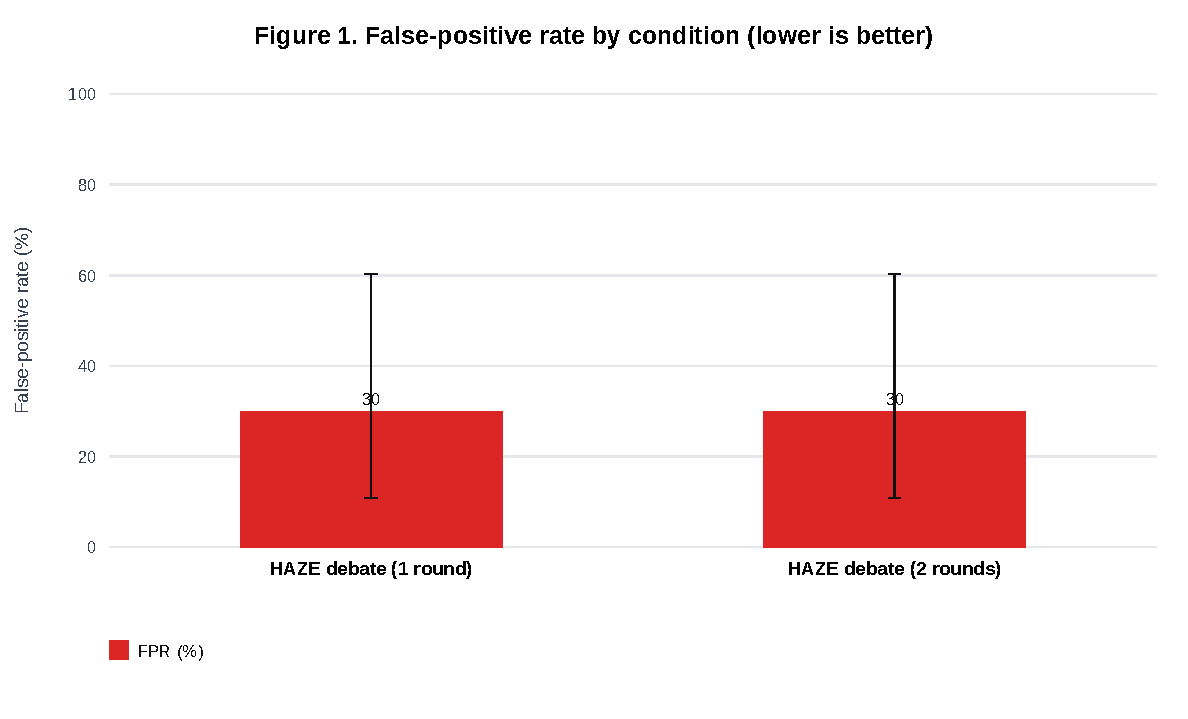
\includegraphics[width=0.92\linewidth]{../evaluation/results/figures/fig1_fpr.pdf}
\caption{False-positive rate by condition (lower is better). Error bars: Wilson 95\% CIs.}
\end{figure}

\begin{figure}[ht]
\centering
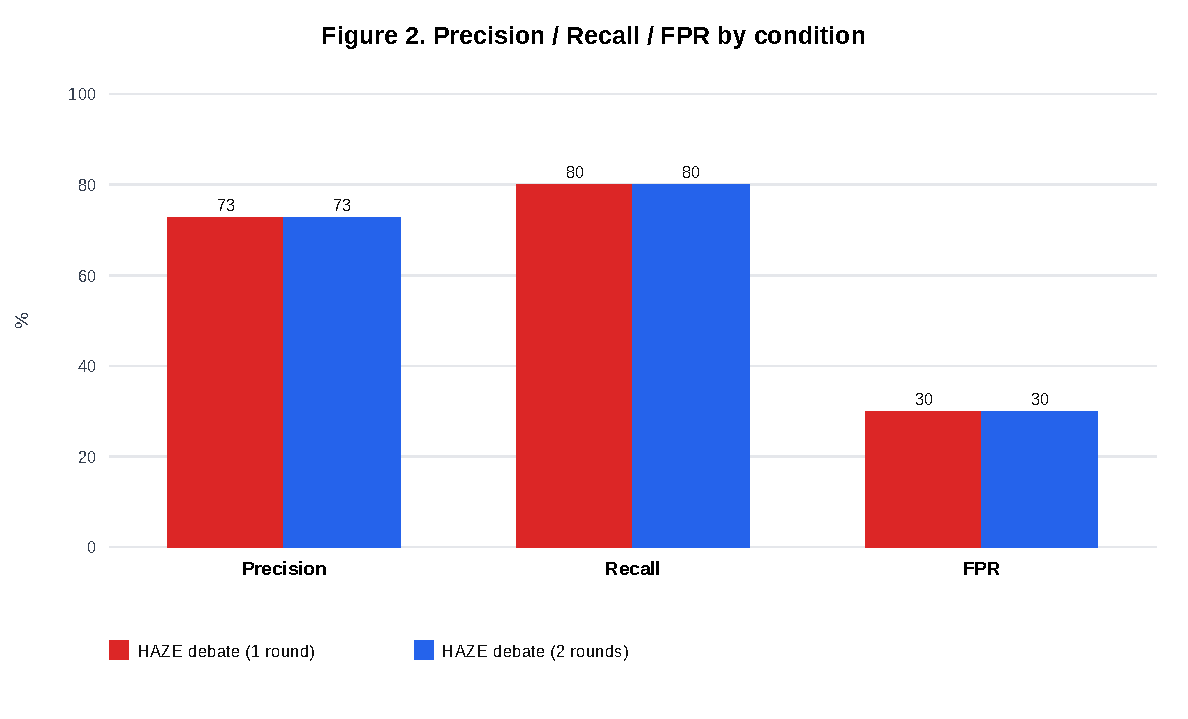
\includegraphics[width=0.92\linewidth]{../evaluation/results/figures/fig2_metrics.pdf}
\caption{Precision, recall, and FPR for 1- vs.\ 2-round HAZE debate.}
\end{figure}

% =============================================================================
\section{Discussion and Limitations}

\textbf{Implications.} HAZE instantiates \textit{scalable oversight}: the judge evaluates
which side survived cross-examination rather than generating the audit from scratch---the
step most prone to hallucination. For pipeline security, structured debate plus full
transcripts supports human review before blocking deployments. OpenRouter access means
teams without local GPUs can run the protocol---relevant for Global South contexts.

\textbf{Validation status.} Table~\ref{tab:validation} separates measured results from
pending experiments. Acknowledging missing controls is necessary but does not substitute
for them; the one-command baseline is shipped as \texttt{run\_phase1.mjs}.

\begin{table}[ht]
\centering
\small
\caption{Measured vs.\ pending experiments (second review, June 2026).}
\label{tab:validation}
\begin{tabularx}{\textwidth}{@{}L{3.2cm} L{2.4cm} L{2.2cm} X@{}}
\toprule
Experiment & Framing & Status & Blocks central claim? \\
\midrule
Web eval (120 tasks) & Malware & Measured & Superseded \\
Single-agent baseline & VULN./SAFE & \textbf{Measured} & No (provides the comparison) \\
HAZE debate (1 round) & VULN./SAFE & \textbf{Measured} & No (provides the result) \\
Benchmark $n{\geq}60$ & VULN./SAFE & Pending & Statistical power \\
\bottomrule
\end{tabularx}
\end{table}

\textbf{Limitations.} (i)~No Investigator or external CVE lookup. (ii)~Judge is still an
LLM. (iii)~Single-file, 24k-char window. (iv)~McNemar $p{=}0.34$ at $n{=}20$---FPR drop
(80\%$\rightarrow$20\%) is \textbf{directional but not statistically significant}; wider
benchmark needed. (v)~Recall trade-off: debate misses 2 cross-file flaws the baseline
``detects'' via over-flagging (100\% recall, 80\% FPR). Unaddressed threats: collusion,
prompt injection, distributed vulnerabilities.

\textbf{Dual use.} HAZE could help adversaries iteratively refine code until it receives
\texttt{SEGURO}, or automate reputational harm via unreviewed \texttt{VULNERABLE} verdicts.
Mitigations: human-in-the-loop before enforcement; no public unauthenticated deployments;
verdicts are decision \textit{aids}, not certificates.

\textbf{Future work.} (1)~Expand benchmark to $n{\geq}60$ for McNemar power.
(2)~Investigator (NVD/OSV). (3)~Multi-file RAG for Class~B blind spots.
(4)~Deploy reframed API to production.

% =============================================================================
\section{Conclusion}

Single-agent auditors ask ``is there a bug?'' and often invent one---our baseline flags
\textbf{80\% of patched code} as vulnerable (100\% recall, 80\% FPR). HAZE asks ``did this
accusation survive refutation?'' and cuts FPR to \textbf{20\%} at 80\% recall and 80\% F1
(Phase~1, \texttt{VULNERABLE}/\texttt{SEGURO}, $n{=}20$). McNemar $p{=}0.34$ means the
effect is promising but underpowered; HAZE remains a reproducible, ${\sim}$USD~0.02/verdict
audit scaffold for AI-control-style oversight in resource-constrained settings.

% =============================================================================
\section*{Reproducibility and Artifacts}

\textbf{One-line summary.} HAZE (\textit{Hallucination-Aware Zero-sum Examination})
is a multi-agent security-audit protocol---2v2 debate plus an isolated judge over
OpenRouter---that reframes the audit question from ``is there a bug?'' to ``did this
accusation survive refutation?''

\textbf{Headline result (Phase~1, measured).} A single-agent auditor flags 80\% of
patched code as vulnerable (100\% recall, 80\% FPR). HAZE lowers FPR to 20\% at
80\% recall and 80\% F1---a 4$\times$ reduction in pipeline-audit hallucinations
(McNemar $p{=}0.34$, $n{=}20$; promising but small-sample).

\textbf{Built and repeatable.} A Fastify monolith with an SSE web UI and an
OpenRouter orchestrator (five-model roster), a 10-CVE benchmark in
\{vulnerable, patched\} variants, the \texttt{run\_phase1.mjs} harness, 120 stored
debate transcripts, and Wilson/McNemar metrics.

\textbf{Reproduce the evaluation} (${\sim}$9~min, ${\sim}$USD~2):
\begin{verbatim}
cd evaluation && node run_phase1.mjs
\end{verbatim}

\textbf{Links.}
\begin{itemize}[leftmargin=*,nosep]
  \item Live demo: \url{https://hackaton.xooktech.com/}
  \item Repository: \url{https://github.com/AXLAAF/V2-Hackathon}
\end{itemize}

\textbf{Submission tracks (AISMX).} AI Security $\rightarrow$ Pipeline security
(API, cloud); Responsible AI $\rightarrow$ Hallucination mitigation \& behavioral
audit. Region: Latin America.

% =============================================================================
\section*{Code and Data}

\begin{itemize}[leftmargin=*,nosep]
  \item \textbf{Repository:} \url{https://github.com/AXLAAF/V2-Hackathon}
  \item \textbf{HAZE tool:} \texttt{API/} --- Fastify backend, OpenRouter orchestrator,
  SSE debate API, web UI
  \item \textbf{Live demo:} \url{https://hackaton.xooktech.com/}
  \item \textbf{Benchmark:} \texttt{vulnerabilities/} --- 10 CVEs $\times$
  \{vulnerable, patched\}
  \item \textbf{Evaluation:} \texttt{evaluation/} --- \texttt{run\_eval.mjs},
  \texttt{analyze.py}; prior web run: 120 transcripts in \texttt{results/}
  \item \textbf{Phase-1 validation:} \texttt{run\_phase1.mjs} --- baseline +
  debate (\texttt{results/raw\_phase1.jsonl})
\end{itemize}

% =============================================================================
\section*{Author Contributions}

Samuel Blanco and Axel Morales --- architecture, API implementation, and orchestration.
Samuel Díaz --- evaluation harness, benchmark, and metrics. Alex Novelo --- writing and
analysis. All authors contributed to the final report.

% =============================================================================
\section*{References}

\begin{enumerate}[leftmargin=*,label={[\arabic*]},nosep,itemsep=0.15em]
  \item Du, Y., Li, S., Torralba, A., Tenenbaum, J. B., \& Mordatch, I. (2023).
  \textit{Improving factuality and reasoning in language models through multiagent debate}.
  arXiv:2305.14325.
  \item Ganguli, D., et al.\ (2022). \textit{Red teaming language models to reduce harms}.
  arXiv:2209.07858.
  \item Irving, G., Christiano, P., \& Amodei, D. (2018). \textit{AI safety via debate}.
  arXiv:1805.00899.
  \item Khan, A., et al.\ (2024). \textit{Debating with more persuasive LLMs leads to more
  truthful answers}. arXiv:2402.06782.
  \item Moe, A., Wale, W., \& Sunde, J. H. (2025). \textit{AI Control through Majority
  Voting}. Apart Research.
  \url{https://apartresearch.com/project/ai-control-through-majority-voting-uiaa}
  \item Perez, E., et al.\ (2022). \textit{Red teaming language models with language models}.
  arXiv:2202.03286.
  \item Zheng, L., et al.\ (2023). \textit{Judging LLM-as-a-Judge with MT-Bench and Chatbot
  Arena}. arXiv:2306.05685.
\end{enumerate}

% =============================================================================
\section*{LLM Usage Statement}

We used LLMs to assist with drafting, structure, and literature framing of this report.
LLMs are also the system under study (the debating agents in HAZE). All technical claims,
cited references, and empirical results were independently verified by the authors. The
final submission was reviewed and edited by the team.

\end{document}
